\documentclass[dvipdfmx,14pt,notheorems,aspectratio=169]{beamer}
%%%% 和文用 %%%%%
\usepackage{bxdpx-beamer}
\usepackage{pxjahyper}
\usepackage{minijs}%和文用
\usepackage{wallpaper}
\usepackage{graphicx, xcolor}
\usepackage{tikz, verbatimbox}
\usetikzlibrary{positioning,shapes,snakes,calc,patterns}
\newcommand{\thickhrulefill}{\leavevmode\leaders\hrule depth-1.2pt height 3.2pt\hfill\kern0pt}
\newcommand{\indicatewidth}[1]{\thickhrulefill{#1}\thickhrulefill}
\input Typocaps.fd
\newcommand*\initfamily{\usefont{U}{Typocaps}{xl}{n}}
\usepackage{foekfont} %font
\usepackage{aurical}
\usepackage[T1]{fontenc}

\renewcommand{\kanjifamilydefault}{\gtdefault}%和文用

%%%% スライドの見た目 %%%%%
\usefonttheme{serif}
\usetheme[numbering=none]{CodeCourse}
\setbeamertemplate{navigation symbols}{}
\setbeamercovered{transparent}%好みに応じてどうぞ)
\setbeamertemplate{footline}[page number]
\setbeamerfont{footline}{size=\normalsize,series=\bfseries}
%%%%

%%%% 定義環境 %%%%%
\usepackage{amsmath,amssymb}
\usepackage{amsthm}
\theoremstyle{definition}
\newtheorem{theorem}{定理}
\newtheorem{definition}{定義}
\newtheorem{proposition}{命題}
\newtheorem{lemma}{補題}
\newtheorem{corollary}{系}
\newtheorem{conjecture}{予想}
\newtheorem*{remark}{Remark}
\renewcommand{\proofname}{}
%%%%%%%%%

%%%%% フォント基本設定 %%%%%
\usepackage[T1]{fontenc}%8bit フォント
%\usepackage[T2A]{fontenc}%8bit フォント
\usepackage{newpxtext}%欧文フォントの追加
\usepackage[utf8]{inputenc}%文字コードをUTF-8
\usepackage{otf}%otfパッケージ
\usepackage{lxfonts}%数式・英文ローマン体を Lxfont にする
\usepackage{bm}%数式太字
%%%%%%%%%%
\usepackage{moreverb}
\usepackage{comment}
\usepackage{url}

\newcommand{\ifexp}[3]{{\rm if}\ {#1}\ {\rm then}\ {#2} \ {\rm else}\ {#3}}
\newcommand{\whileexp}[2]{{\rm while}\ {#1}\ {\rm do}\ {#2}}
\newcommand{\skipexp}{{\rm skip}}
\newcommand{\failexp}{{\rm fail}}
\newcommand{\returnexp}[1]{{\rm return}\ {#1}}
\newcommand{\evalexp}[2]{{\rm eval}({#1},\, {#2})}
\newcommand{\callexp}[1]{{\rm call}({#1})}
\newcommand{\substexp}[2]{\texttt{{#1}:=\,{#2}}}
\newcommand{\judge}[3]{\vdash {#1} : {#2} \ast {#3}}


\title[]{誰も知らない OCaml\\{\small 僕も知らない}}%[略タイトル]{タイトル}
\author[]{\large KMCID: taisei}%[略名前]{名前}
%\institute[]{B4}%[略所属]{所属}
\date{5/9/2022}%日付

\begin{document}
    
    \setbeamertemplate{background}
    {
        %\begin{centering}
        %	\includegraphics[width=\paperwidth]{mountain.jpg}
        %\end{centering}
    }
    \begin{frame}
    \titlepage %表紙
    \end{frame}
    \setbeamertemplate{background}
    {
    
    }

    \setbeamertemplate{background}
    {
        \begin{centering}
            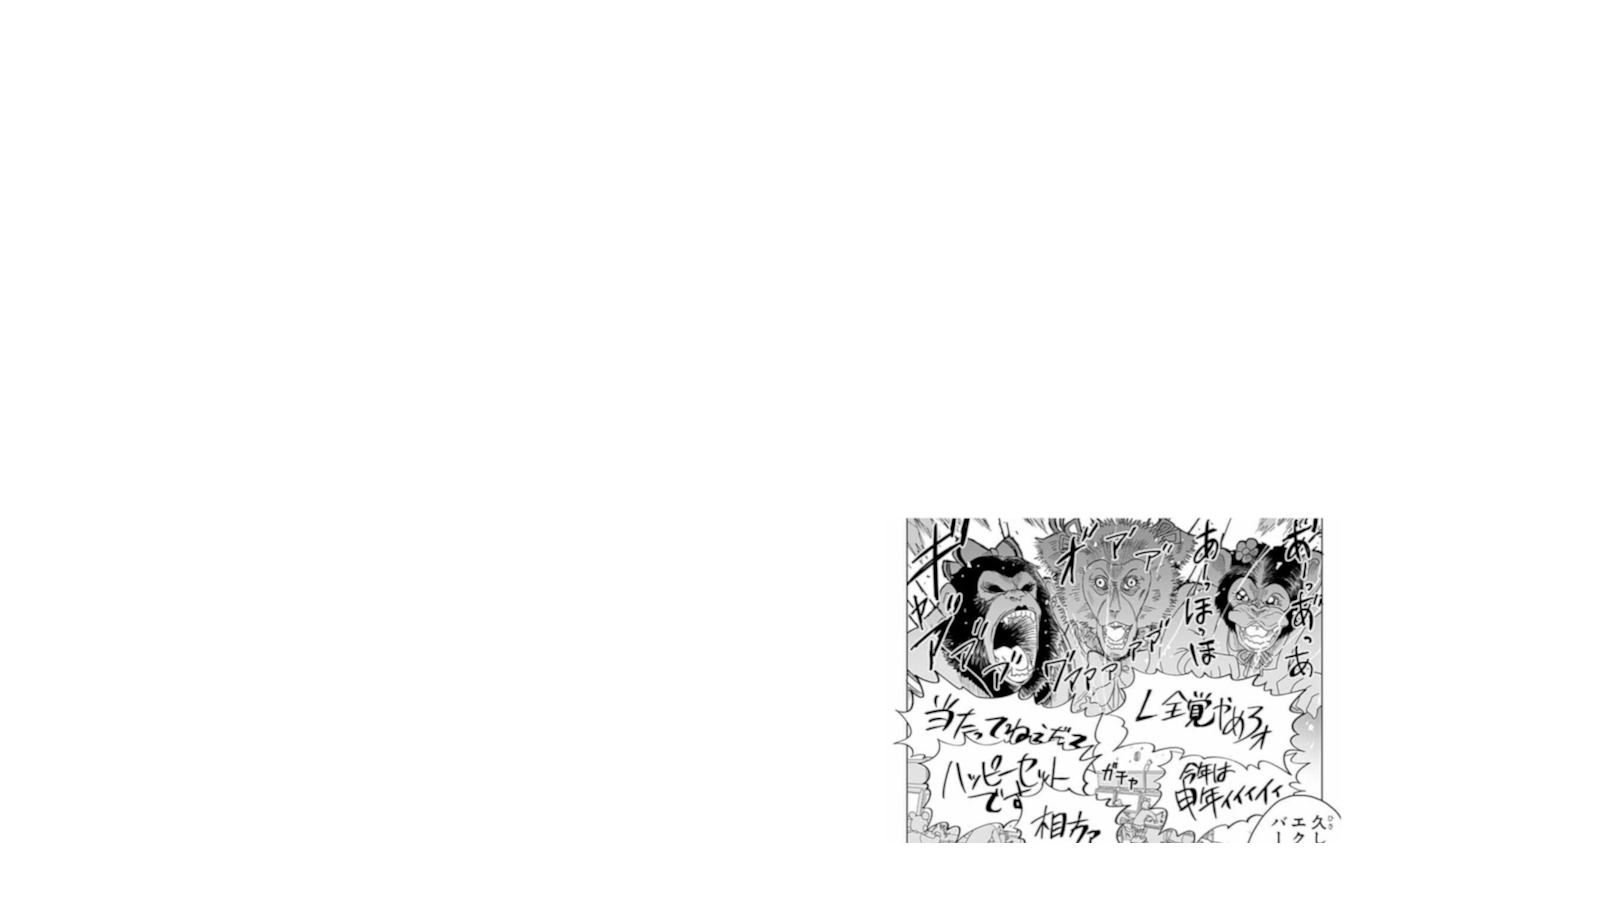
\includegraphics[width=\paperwidth]{chimpanzee.png}
        \end{centering}
    }
    \begin{frame}[fragile]\frametitle{自己紹介}
        KMCID: taisei
        \begin{itemize}
            \item たしか39代副会長
            \item 京大工情報計算機 $\rightarrow$ 京大院情報学研究科通信情報システム \\
            $\rightarrow$ 京都在住エンジニャ
            \item 競プロCTF中退
            \item EXVS猿\footnote{出典: ゲーミングお嬢様}
        \end{itemize}
    \end{frame}
    \setbeamertemplate{background}
    {}

\begin{comment}
    \begin{frame}[fragile]\frametitle{近況}
        \begin{itemize}
            \item 昨日しまなみ海道を走ってきました
        \end{itemize}
    \end{frame}
    \setbeamertemplate{background}
    {}
\end{comment}

    \begin{frame}[fragile]\frametitle{やること}
        \begin{itemize}
            \item ここ数年 OCaml ばっかり書いてる
            \item ここ数年で言語の更新や新機能の追加が加速した気がする
            \item OCaml 書いててこんなんできるんだ〜ってなったを紹介
        \end{itemize}
        \begin{figure}[htbp]
            \begin{center}
                
\includegraphics[width=3cm]{camel.jpeg}
            \end{center}
        \end{figure}
    \end{frame}

    \begin{frame}[fragile]\frametitle{OCaml}
        \begin{itemize}
            \item OCaml \footnote{知らない人は \cite{igarashi}, \cite{ksuenaga} 辺りを参照} : Objective Caml
            \begin{itemize}
                \item Caml : Categorical Abstruct Machine Language \footnote{Meta Languageだと思っていたけれど違った}らしい
            \end{itemize}
            \item ML\footnote{Machine Learning ではない} 方言 関数型プログラミング言語の一つに分類されがち
            \item 計算機コースの人は必修
        \end{itemize}
    \end{frame}

    \begin{frame}[fragile]\frametitle{こんなの}
        \begin{exampleblock}{適当な例1}
            \scriptsize
            \begin{verbatimtab}
type point = { x: int; y: int } (* x, y を持つ record の宣言 *)
(* 2つの point を持つ Square と, point と int を持つ Circle の variant *)
type shape = Square of point * point | Circle of point * int 
let pi = 4.0 *. atan 1.0 (* 定数定義 *)
let area sp = match sp with (* 関数定義. sp が Shape か Cirle かで分岐 *)
    | Square ({x=px; y=py}, q) -> float_of_int ((q.y-py) * (q.x-px))
    | Circle (_, r) -> let r = float_of_int r in r *. r *. pi
\end{verbatimtab}
        \end{exampleblock}
        Circle と Square の 2 種類の shape を定義し, shape の面積を求める関数 area を定義
    \end{frame}

    \begin{frame}[fragile]\frametitle{こんなの}
        \begin{exampleblock}{適当な例2}
            \scriptsize
            \begin{verbatimtab}
module List = struct
    type 'a list = Nil | Cons of 'a * 'a list (* 多相型 *)
    let rec map : ('a -> 'b) -> 'a list -> 'b list = (* 再帰関数定義 *)
        fun f -> function
        | Nil -> Nil
        | Cons (h, t) -> Cons (f h, map f t)
end
let double_list : int List.list -> int List.list =
    List.map (fun x -> x * 2) (* 部分適用 *)
\end{verbatimtab}
        \end{exampleblock}
        \footnote{function は fun x -> match x with の構文糖衣}
        関数 map を持つモジュール List を定義し, List で定義したリストの各要素を2倍にする関数 double\_list を定義
    \end{frame}

    \begin{frame}[fragile]\frametitle{もくじ}
        \begin{itemize}
            \item Extensible Variant Type
            \item Polymorphic Variant
            \item Monadic bind
            \item PPX
            \item Type Construct over Signatures \& Substituting inside a Signature
        \end{itemize}
    \end{frame}

    \begin{frame}[fragile]\frametitle{Extensible Variant Type}
        \begin{itemize}
            \item コンストラクタを後で追加できる(???)
        \end{itemize}
        \begin{exampleblock}{Extensible Variant Type}
            \scriptsize
            \begin{verbatimtab}
type t = .. (* 省略していません!! *)
type t += Str of string
type t +=
    | Int of int
    | Float of float
\end{verbatimtab}
        \end{exampleblock}
    \end{frame}


    \begin{frame}[fragile]\frametitle{Extensible Variant Type}
        \begin{itemize}
            \item よく Result モナドの Error.t 型の方で使われる
        \end{itemize}
        \begin{exampleblock}{Extensible Variant Type}
            \scriptsize
            \begin{verbatimtab}
module Error = struct
    type t = ..
    type t += Fatal of string
end
type 'a result = Ok of 'a | Error of Error.t

module Arith = struct
    type Error.t += Overflow | ZeroDivision
    let div a b = if b = 0 then (Error ZeroDivision) else Ok (a/b)
end
\end{verbatimtab}
        \end{exampleblock}
    \end{frame}

    \begin{frame}[fragile]\frametitle{Polymorphic Variant}
        \begin{itemize}
            \item どの型にも属さないコンストラクタ 通称タグ
            \begin{itemize}
                \item 先頭が `(バッククォート) で始まる
            \end{itemize}
            \item 型宣言なしで使えるが, 型注釈してもよい
            \begin{itemize}
                \item pattern-match で便利になるかも
            \end{itemize}
        \end{itemize}
        \begin{exampleblock}{Polymorphic Variant}
            \scriptsize
            \begin{verbatimtab}
type myvariant = [`Tag1 of int | `Tag2 of bool]
let f = function
    | #myvariant -> "myvariant" (* myvariant 型に属する tag 全てにマッチ *)
    | `Tag3 -> "Tag3"
======
val f : [< `Tag1 of int | `Tag2 of bool | `Tag3 ] -> string
\end{verbatimtab}
        \end{exampleblock}
    \end{frame}

    \begin{frame}[fragile]\frametitle{Polymorphic Variant}
        \begin{itemize}
            \item \lbrack \textless .. \rbrack : サブセットを表す型
            \item \lbrack \textgreater .. \rbrack : スーパーセットを表す型
        \end{itemize}
        \begin{exampleblock}{Polymorphic Variant}
            \scriptsize
            \begin{verbatimtab}
type t = [`A | `B | `C]
let f = function
    | #t as t -> t
    | `D -> `E
let g = function
    | #t as t -> t
    | x -> x
======
val f : [< `A | `B | `C | `D ] -> [> `A | `B | `C | `E ] = <fun>
val g : ([> t ] as 'a) -> 'a = <fun>
\end{verbatimtab}
        \end{exampleblock}
    \end{frame}

\begin{comment}
    \begin{frame}[fragile]\frametitle{Polymorphic Variant}
        \begin{itemize}
            \item module abstract type に polymorphic variant を含む型が与えられたときにどう解釈するかを,
            type +'a, -'b とかで与えられる
            \url{https://blog.janestreet.com/a-and-a/}
        \end{itemize}
        \begin{exampleblock}{Polymorphic Variant}
            \scriptsize
            \begin{verbatimtab}
\end{verbatimtab}
        \end{exampleblock}
    \end{frame}
\end{comment}


\begin{frame}[fragile]\frametitle{Monadic Bind}
    \begin{itemize}
        \item これまで OCaml で Monad を書くと bind 演算子祭りになって辛かった
        \begin{itemize}
            \item 関数がネストして見辛い
            \item 型が合わないエラー等の場所が分かりづらくなっていた
        \end{itemize}
    \end{itemize}
    \begin{exampleblock}{Monadic Bind}
        \scriptsize
        \begin{verbatimtab}
let bind x f = match x with Some x -> f x | None -> None
let both x y = match (x, y) with Some x, Some y -> Some (x, y) | _ -> None
let return x = Some x
let (>>=) = bind

both (return 1) (return 2) >>= (fun (x, y) ->
return 3 >>= (fun z ->
return (x + y + z)))\end{verbatimtab}
    \end{exampleblock}
\end{frame}

    \begin{frame}[fragile]\frametitle{Monadic Bind}
        \begin{itemize}
            \item let(symbol+) と and(symbol+) を演算子として定義できる
            \item let文っぽく書いて特殊な感じで展開してくれる
        \end{itemize}
        \begin{exampleblock}{Monadic Bind}
            \scriptsize
            \begin{verbatimtab}
let (let*) = bind
let (and*) = both

let* x = return 1 and* y = return 2 in
let* z = return 3 in
return (x + y + z)

 : (* 展開されると *)

(let*) ((and*) (return 1) (return 2)) (fun (x, y) ->
(let*) (return 3) (fun z ->
return (x + y + z)))\end{verbatimtab}
        \end{exampleblock}
    \end{frame}


    \begin{frame}[fragile]\frametitle{PPX (PreProcessor eXtension)\cite{ppx}}
        {\small
        \begin{itemize}
            \item literal, attribute, extension point を埋め込める
            \item コードの AST から AST へ変換する関数を前処理で実行できる
            \begin{itemize}
                \item 型付け前なので型情報は無い
            \end{itemize}
            \item  マクロ, リテラル, コード生成, monadic なキーワード定義などに
        \end{itemize}
        }
        \begin{exampleblock}{ppx}
            \scriptsize
            \begin{verbatimtab}
123456z ==> Z.of_int 123456 (* literal. 多倍長整数へ変換 *)

type point3d = float * float * float
[@@deriving show] (* attribute. show 関数を自動定義 *)

match%lwt x with ... ==> [%lwt match x with ...] (* exptention point *)
==> Lwt.bind x (function ...) (* モナドで持ち上がった x を展開 *)\end{verbatimtab}
        \end{exampleblock}
    \end{frame}


    \begin{frame}[fragile]\frametitle{Type Construct Over Signatures\footnote{それっぽい呼び方見つからなかったので適当につけた}}
        \begin{itemize}
            \item module名 with type t = u とすると, 型同士の制約を追記できる
        \end{itemize}
        \begin{exampleblock}{Type Construct over signatures}
            \scriptsize
            \begin{verbatimtab}
module type Monad = sig
    type 'a t (* 抽象型 *)
    val return : 'a -> 'a t
    val bind : 'a t -> ('a -> 'b t) -> 'b t
end
module type OptionMonad : Monad with type 'a t = 'a option
======
module type OptionMonad = sig
    type 'a t = 'a option
    val return : 'a -> 'a t
    val bind : 'a t -> ('a -> 'b t) -> 'b t
  end\end{verbatimtab}
        \end{exampleblock}
    \end{frame}


    \begin{frame}[fragile]\frametitle{Substituting inside a Signature}
        \begin{itemize}
            \item module名 with type t := u とすると, t を uで書き換える(??)
            \footnote{最近 module type を module type で代入できるようになった(??)}
        \end{itemize}
        \begin{exampleblock}{Substituting inside a signature}
            \scriptsize
            \begin{verbatimtab}
module type Monad = sig
    type 'a t (* 抽象型 *)
    val return : 'a -> 'a t
    val bind : 'a t -> ('a -> 'b t) -> 'b t
end
module type OptionMonad : Monad with type 'a t := 'a option
======
module type OptionMonad = sig
    val return : 'a -> 'a option
    val bind : 'a option -> ('a -> 'b option) -> 'b option
  end\end{verbatimtab}
        \end{exampleblock}
    \end{frame}

    \begin{frame}[fragile]\frametitle{紹介しなかったトピック}
        \begin{itemize}
            \item OCaml の O の部分
            \begin{itemize}
                \item 未だに書いたこと無い...
            \end{itemize}
            \item GADT \cite{gadt}
            \begin{itemize}
                \item Explicit polymorphic Annotations + Locally Abstract Type の謎記法
            \end{itemize}
            \item Pretty Printer\cite{pp}
        \end{itemize}
    \end{frame}

    \begin{frame}[fragile]\frametitle{最後に}
        \begin{block}{Quiz}
            \scriptsize
        \begin{verbatimtab}
type _ expr =
| Int : int -> int expr
| Add : (int -> int -> int) expr
| App : ('a -> 'b) expr * 'a expr -> 'b expr

let rec eval [% ??? ] = function
| Int n -> n
| Add -> (+)
| App (f, x) -> eval f (eval x)\end{verbatimtab}
        \end{block}
        \lbrack \% ??? \rbrack に入れてコンパイルが通るのは次のうちどれでしょう?
    \end{frame}

    \begin{frame}[fragile]\frametitle{最後に}
        \begin{enumerate}[1]
            \item (type t) : t expr -> t
            \item : type t. t expr -> t
            \item : t. t expr -> t
            \item : 't. 't expr -> 't
            \item 実は何も書かなくてもいける
        \end{enumerate}
    \end{frame}

    \begin{frame}[allowframebreaks]\frametitle{\foekfamily REFERENCES}
        \bibliographystyle{plain}
        \bibliography{bibliography/bibliography}
        \begin{thebibliography}{99}
        \beamertemplatetextbibitems
        \bibitem{RR} \url{https://ocaml.org/manual/index.html}
        \bibitem{igarashi} \url{https://hackmd.io/@aigarashi/r1az0wOHP/\%2FBsXrOToESu-Q30kiM_PAmg}
        \bibitem{ksuenaga} \url{https://github.com/kuis-isle3sw/IoPLMaterials/blob/master/textbook/slides/ocaml.pdf}
        \bibitem{ppx} \url{https://dailambda.jp/slides/2021-04-09-ppx.html\#/what-is-ppx-1}
        \bibitem{gadt} \url{https://www.math.nagoya-u.ac.jp/~garrigue/papers/ml2011-show.pdf}
        \bibitem{pp} \url{https://qnighy.hatenablog.com/entry/2017/01/26/215948}
        \end{thebibliography}
    \end{frame}


\end{document}
